\section{Intel Quantum Simulator on Kay}
\label{sec:intel_quantum_simulator_on_kay}

%---------------------------------------------------------------------------------
\subsection{Installation Setup}
\label{sec:installation_setup}
ICHEC's primary supercomputer Kay was installed in August 2018 and is comprised of
\begin{itemize}
    \item 336 node cluster.
    \item 13,440 CPU cores, 63 TB distributed memory.
    \item Dual-socket 20-core Intel® Xeon Gold (Skylake) 6148 at 2.4 GHz with 192 GB memory.
    \item 400 GB local SSD scratch.
    \item 100 GB Intel® OmniPath network.
    \item Additional partitions
    \begin{itemize}
        \item Intel Xeon Phi (Knights Landing architecture).
        \item High-memory 1.5 TB RAM with 1TB local SSD scratch.
        \item Dual NVIDIA Tesla V100.
    \end{itemize}
\end{itemize}

The \textit{master} branch of the Intel Quantum Simulator from the \textit{intel/Intel-QS} GitHub repository was installed on Kay in the path 
\begin{verbatim}
/ichec/work/ichec001/
\end{verbatim}

 Intel Parallel Studio XE 2018 update 4 was used as the default MPI compiler. Vectorisation was enabled using AVX512 instead of the default SSE2.

%---------------------------------------------------------------------------------
\subsection{Performance and Scaling}
\label{sec:performance_and_scaling}
Testing was conducted using the \textit{/tests/qft\_test.cpp} application supplied with the simulator which conducted a quantum Fourier transform using a specified number of qubits. Experiments were conducted for this application to demonstrate its weak and strong scaling performance. Many applications for quantum simulators are subject to being memory bound and under certain circumstances compute bound. Due to the large memory footprint of the number of states which doubles as the number of qubits increases by one, and the overhead of the corresponding access of that memory, the application was expected to be memory bound, and thus have relatively good weak scaling performance. As the number of quantum gate operations is increased in a quantum circuit the number of classical gates required to conduct the simulation can increase very quickly since these quantum gates are applied to an increasing number of qubits. Therefore, as the number of qubits are increased, the number of classical operations would increase significantly. Thus applications on the Intel Quantum Simulator are also subject to being compute bound.

Table \ref{tab:scaling_experiment_config} details the configuration of each experiment for both strong and weak scaling using double and also single precision numbers to represent the states. Figure \ref{fig:strong_scaling} illustrates the results of the strong scaling performance and figure \ref{fig:weak_scaling} that of the weak scaling experiments.
Both figure \ref{fig:strong_scaling} and figure \ref{fig:weak_scaling} appear to scale approximately in a linear fashion. This implies that the application scaled relatively well for both weak and strong scaling. However, it would be desirable to conduct more experiments for larger problem sizes to further observe the scalability of the application. This was not possible due to a limit on the maximum MPI message size preventing larger problem sizes of approximately $2^{27}$ double precision states per process. Thus the simulator could not be tested up to the maximum available memory on a node. 
% It must also be noted that the double precision performance for weak scaling was notably worse than that of single precision. However, it appears to perform worse by approximately the addition of a constant, which does not prove to be a significant issue.

\begin{table}[H]
    \begin{tabular}{|c|c|c||c|c||c|c|}
        \hline
        \multicolumn{3}{|c||}{Scaling} & \multicolumn{2}{|c||}{Strong} & \multicolumn{2}{|c|}{Weak}\\
        \hline
        Nodes           &  p    & NumProcs   & Local States  & Qubits      & Local States & Qubits \\
                   &     &  $2^p$  &  $ 2^{n-p}$  &   $n$      & $ 2^{n-p} = 2^{27}$ &  $n$\\
    
        \hline
        64              &   7   & 128                   & $2^{28-7}$                        & 28         & $2^{34-7}$& 34 \\
        32              &   6   & 64                    & $2^{28-6}$                         & 28        &$2^{33-6}$&  33 \\
        16              &   5   & 32                    & $2^{28-5}$                         & 28        &$2^{32-5}$&  32 \\
        8               &   4   & 16                    & $2^{28-4}$                         & 28        &$2^{31-4}$&  31 \\
        4               &   3   & 8                     & $2^{28-3}$                         & 28        &$2^{30-3}$&  30 \\
        2               &   2   & 4                     & $2^{28-2}$                         & 28        &$2^{29-2}$&  29 \\
        1               &   1   & 2                     & $2^{28-1}$                        & 28         &$2^{28-1}$&  28\\
     \hline
    \end{tabular}
    \caption{Details of number of total qubits, and local number of states per process for the corresponding experiment for both strong and weak scaling. }
    \label{tab:scaling_experiment_config}
\end{table}

\begin{figure}[H]
	\centering
	\begin{minipage}{.5\linewidth}
		\centering
		%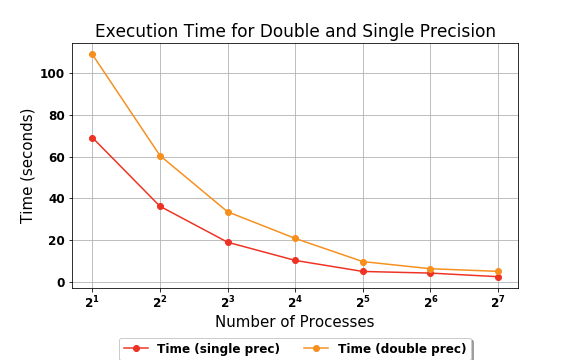
\includegraphics[width=1.\linewidth]{scaling_strong_log2.png}
		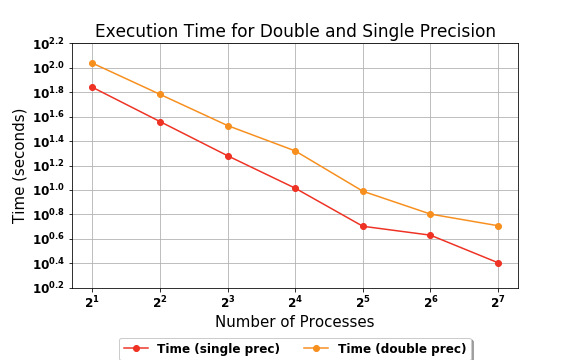
\includegraphics[width=1.\linewidth]{scaling_strong_log2log10.png}
		\caption{Strong scaling of execution time.}
		\label{fig:strong_scaling}
	\end{minipage}%
	\begin{minipage}{.5\linewidth}
		\centering
		%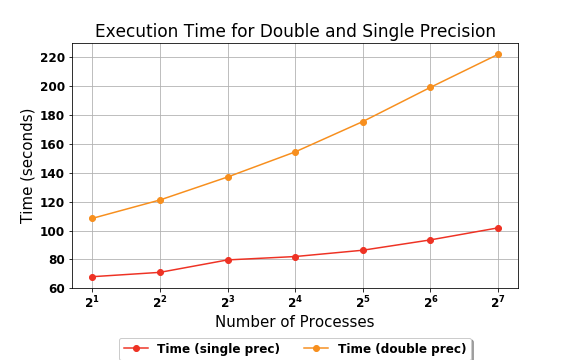
\includegraphics[width=1.\linewidth]{scaling_weak_log2.png}
		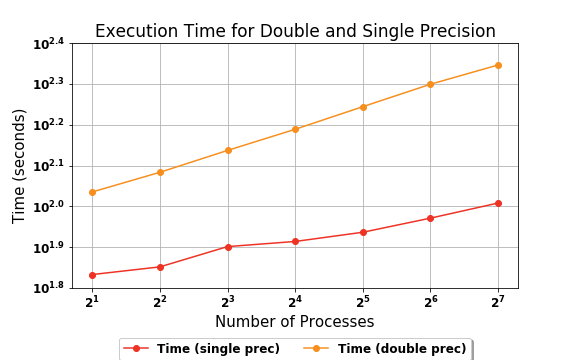
\includegraphics[width=1.\linewidth]{scaling_weak_log2log10.png}
		\caption{Weak scaling of execution time.}
		\label{fig:weak_scaling}
	\end{minipage}
\end{figure}